\documentclass[a4paper, 12pt]{report}

\usepackage{lmodern} % Police standard sous LaTeX : Latin
\usepackage[english]{babel} % Pour la langue anglaise
\usepackage[utf8]{inputenc} % Pour l'UTF-8
\usepackage[T1]{fontenc} % Pour les césures des caractères
\usepackage{graphicx}
\usepackage{subfig}
\usepackage{ragged2e}
\justifying

\renewcommand{\thesection}{\Alph{section}}

\title{Model of the spread of a disease in a population of mobile agents}
\author{NIDDAM Benjamin}
\date{\today}

\begin{document}
\begin{titlepage}
	\maketitle
\end{titlepage}

\newpage

\tableofcontents

\newpage
\section{Introduction}

Après la découverte d'une nouvelle maladie, on cherche à étudier son comportement sur une population d'agents mobiles.
Dans un second temps, on étudiera différentes stratégies pour endiguer sa propagation. On veut donc, à la fin,
connaitre le ou les moyens les plus efficaces pour éviter que la maladie ne se propage dans la population.

\section{Model presentation}
\subsection{Variables definition}

La première étape consiste à définir les différents paramètres de la simulation. Nous aurons donc:
\begin{itemize}
	\item une durée de simulation
	\item un nombre d'agents
	\item un nombre d'agents contaminés au temps zéro
	\item un degrés de confinement de la population
	\item un degrés de de respect des gestes barrières
\end{itemize}

\subsection{Agents presentation}

Nos agents sont représentés par des cercles de coordonnées (x, y) et de rayon (r). Ils possèdent un état de contamination booléen, une probabilité de contamination (p), un état de guérison booléen et un état d'imunité boolean. Ces états sont modifiés par les interactions entre les agents et des durées définies qui cherchent à être les plus proches de la réalité. Les agents évoluent dans un monde carré de dimension (w, h) et sont placés aléatoirement dans ce monde avec une vitesse (vx, vy), elle aussi aléatoire.

\subsection{interactions definition}

Il n'existe qu'un seul type d'interaction entre nos agents. C'est l'interaction de contagion. Lorsqu'un agent est contaminé, il peut infecter d'autres agents mais ne peut plus être contaminé. Pour qu'un agent sain se fasse contaminé, il doit respecter certaines conditions. Il doit être un rayon de contamination (ir) défini. Il doit être sain, ne pas être immunisé et ne pas être vacciné.

\begin{figure}[h]
	\centering
	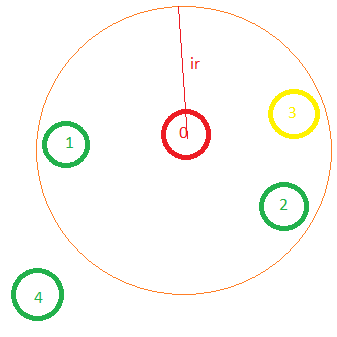
\includegraphics[width=0.5\textwidth]{./Interactions.png}
	\caption{Interaction between agents}
\end{figure}

In this exemple, only the agents in the infection radius (ir) can be infected, only if their not immune(yellow) or infected(red).

% \newpage
\newpage


\section{Experiments, results and limitations}
\subsection{initial state}

In all of our simulations, we used a number of agents fixed to 1000, a number of contaminated agents fixed to 1 and 100 and a 3.5\% contamination degree.
Before starting the tests to contain the disease, we simulated the the evolution of the infecteds agents without any intervention.
Here are the results:

\begin{figure}[h]

	\centering
	\subfloat[\centering 1 infected agent at t0]{{\includegraphics[width=6cm]{../Courbes/1000_agents_1_contaminé_5_ans/Natural_immunity_only.png} }}
	\qquad
	\subfloat[\centering 100 infecteds agents at t0]{{\includegraphics[width=6cm]{../Courbes/1000_agents_100_contaminé_5_ans/Natural_immunity_only.png} }}
	\centering
	\caption{Graphic representations of the evolution of the condition of the population as a function of time}

\end{figure}

The infecteds evolution is represented by a succesion of contamination and healing waves that spread until the end of the simulation. These waves are due to the fact that our agents
gain a temporary immunity after each healing.

\vspace{0.8cm}

There are various expériences that we have done trying to contain or eradicate the disease. For each of these experiments, we simulated it four times with the same initial conditions
and used the average of the results as a representative result to reduce the uncertainty due to randomness.

\newpage

\subsection{Confinement}
Comme première expérience nous avons décidé de confiner la population. Pour ce faire nous divisons les
valeurs de vx et vy par deux, puis par trois et enfin par cinq. Ce qui nous ramène à trois tests que nous
appelons respectivement "confinement léger", "confinement moyen" et "confinement strict" par rapport à leur
taux de limitation. Ce taux fera baisser la possibilité de déplacement des agents jusqu'à la quasi-immobilité
lorsque ce dernier vaut cinq. Ceci entraine donc une réduction des interactions entre les agents qui devrait
limiter la dispersion de la maladie. On veut savoir si cette réduction est suffisante pour éradiquer la maladie. Et
si oui, quel taux faut-il mettre en place et sûr combien de temps. Nous avons donc réalisé les simulations
suivantes:

\begin{figure}[h]
	\centering
	\subfloat[\centering Light confinement]{{\includegraphics[width=6cm]{../Courbes/1000_agents_1_contaminé_5_ans/Light_confinement.png} }}
	\qquad
	\subfloat[\centering Basic confinement]{{\includegraphics[width=6cm]{../Courbes/1000_agents_1_contaminé_5_ans/Partial_confinement.png} }}
	\centering
	\subfloat[\centering Heavy confinement]{{\includegraphics[width=6cm]{../Courbes/1000_agents_1_contaminé_5_ans/Strict_confinement.png} }}
	\qquad
	\caption{Représentations graphique de l'évolution de l'état\\ de la population en fonction du taux de confinement}

\end{figure}
\newpage

Les graphiques ci-dessus représentent l'évolution de l'état des agents au cours de la simulation (temps en jour)en fonction du taux de confinement.
On observe que la méthode de confinement est une facon très efficace de ralentir le déplacement de la maladie au sein de la population. On le constate clairement
sur les graphiques du confinement léger et moyen. En effet, le pic de contamination initial est beaucoup moins important que celui de la simulation sans restrictions.
Enfin, en se basant sur la courbe du confinement stricte, on confirme que cette méthode, malgré un degré très important de limitations, n'est pas suffisante pour éradiquer la maladie.
On peut donc envisager de combiner cette dernière avec une autre méthode. Mais avant cela, nous avons testé si mettre en place un confinement de la population alors que l'épidémie' s'est déja propagée.
Nous obtenons donc les résultats suivants:

\begin{figure}[h]
	\centering
	\subfloat[\centering Light confinement]{{\includegraphics[width=6cm]{../Courbes/1000_agents_100_contaminé_5_ans/Light_confinement.png} }}
	\qquad
	\subfloat[\centering Basic confinement]{{\includegraphics[width=6cm]{../Courbes/1000_agents_100_contaminé_5_ans/Partial_confinement.png} }}
	\centering
	\subfloat[\centering Heavy confinement]{{\includegraphics[width=6cm]{../Courbes/1000_agents_100_contaminé_5_ans/Strict_confinement.png} }}
	\qquad
	\caption{Représentations graphique de l'évolution de l'état\\ de la population en fonction du taux de confinement}

\end{figure}

Grace à ce deuxième set de simmulations, il apparait que lorsque le confinement est décrété dès les premiers cas, on remarque qu'il n'y a aucun pic de contamination quelque soit le taux de confinement.
En comparaison avec les simulation ou le confinement débute avec 10\% de la population infectée, dans lequelles le confinement ne permet que
de dimminuer le premier pic de contamination. Sur le long terme le confinement quelque soit soit sont inensité, permet de stabilser le nombre d'infectés journalier.

\newpage

\subsection{Respect des gestes barrières}
Dans un deuxième temps, nous avons décidé de mettre en place un respect des gestes barrières. Cette méthode cherche à réduire la probabilité qu'un agent contaminé transmette la maladie à un autre agent
lors de leur rencontre. Pour ce faire, nous avons mit en place trois intensités: "Basics barrier gestures", "Mediums barrier gestures" et "Heavys barrier gestures" qui réduisent par deux, trois et cinq
la probabilité d'infection. Dans ce cas, on veut savoir jusqu'à quel niveau les gestes barrières peuvent ralentir la maladie.

\begin{figure}[h]
	\centering
	\subfloat[\centering Light confinement]{{\includegraphics[width=6cm]{../Courbes/1000_agents_1_contaminé_5_ans/Light_confinement.png} }}
	\qquad
	\subfloat[\centering Basic confinement]{{\includegraphics[width=6cm]{../Courbes/1000_agents_1_contaminé_5_ans/Partial_confinement.png} }}
	\centering
	\subfloat[\centering Heavy confinement]{{\includegraphics[width=6cm]{../Courbes/1000_agents_1_contaminé_5_ans/Strict_confinement.png} }}
	\qquad
	\caption{Représentations graphique de l'évolution de l'état\\ de la population en fonction du taux de gestes barrières}

\end{figure}

\newpage

Ici, nous représentons l'évolution de l'état des agents au fil du temps (en jour) en fonction du degrés de respect de la population pour les gestes barrières.
On voit clairement que les gestes barrières sont très efficaces pour réduire la transmission de la maladie même si les agents ne les suivent pas de manière stricte comme le montre le graphique
"gestes barrières basiques".
Grace au courbes, il est clair que les gestes barrières sont une très bonne
pratique pour réduire la transmission de la maladie. De plus, comme le montre le graphique"gestes barrières strictes", si respectés sérieusement et dès les premiers jours, une épidémie peut facilement
être évitée. Mais on peut aussi se demander si cette méthode serait aussi utile, si mise en place alors que l'épidémie est déjà en cours. Voici donc les résultats obtenus pour ce cas:

\begin{figure}[h]
	\centering
	\subfloat[\centering Light confinement]{{\includegraphics[width=6cm]{../Courbes/1000_agents_100_contaminé_5_ans/Light_confinement.png} }}
	\qquad
	\subfloat[\centering Basic confinement]{{\includegraphics[width=6cm]{../Courbes/1000_agents_100_contaminé_5_ans/Partial_confinement.png} }}
	\centering
	\subfloat[\centering Heavy confinement]{{\includegraphics[width=6cm]{../Courbes/1000_agents_100_contaminé_5_ans/Strict_confinement.png} }}
	\qquad
	\caption{Représentations graphique de l'évolution de l'état\\ de la population en fonction du taux de confinement}

\end{figure}

\newpage

Dans le cas présent, le développement de la maladie est atténué par les gestes barrières. Cependant, comme pour l'expérience précédente, à part lorsque les gestes barrières sont fortement respectés,
l'épdiémie n'est pas évitée.

\newpage

\subsection{Vaccination}

Nous avons ensuite instauré un cycle de vaccination. En effet, dans la simulation, chaque jour, nous vaccinons un nombre d'agents définits au préalable.Le vaccin donne une imunité plus longue que celle obtenue
naturellement. Au seins même de cette expérience nous avons pu tester plusieurs choses. Dans un premier temps, les agents n'effectuent qu'une seule vaccination qui les imunisent un certain temps mais finissent
par attraper la maladie à la fin de leur prériode de vaccination.

\begin{figure}[h]
	\centering
	\subfloat[\centering 1 vaccination par jour]{{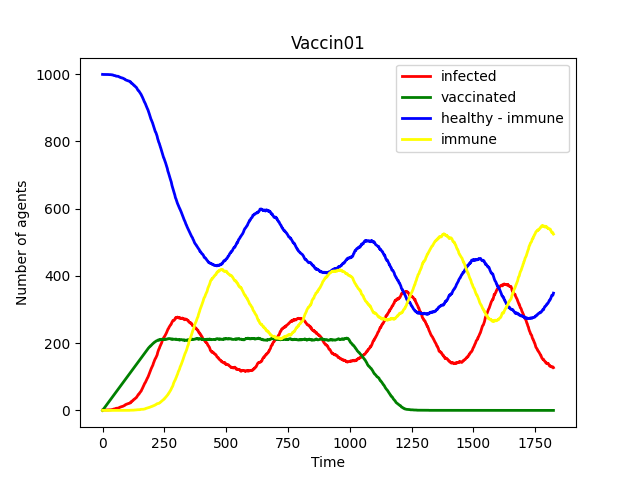
\includegraphics[width=6cm]{../Courbes/1000_agents_1_contaminé_5_ans/Vaccin01.png} }}
	\qquad
	\subfloat[\centering 3 vaccination par jour]{{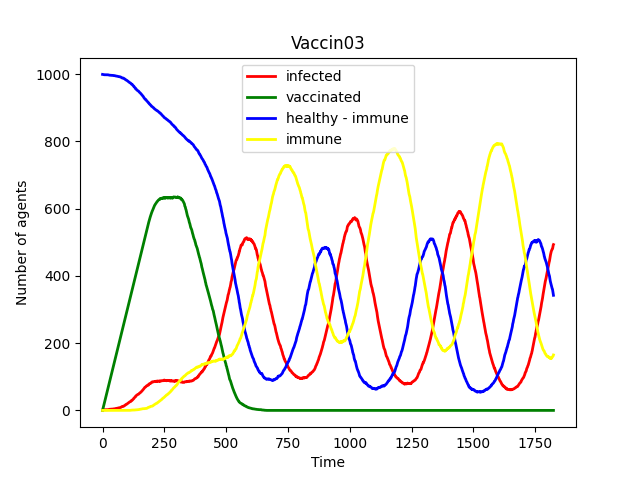
\includegraphics[width=6cm]{../Courbes/1000_agents_1_contaminé_5_ans/Vaccin03.png} }}
	\centering
	\subfloat[\centering 4 vaccination par jour]{{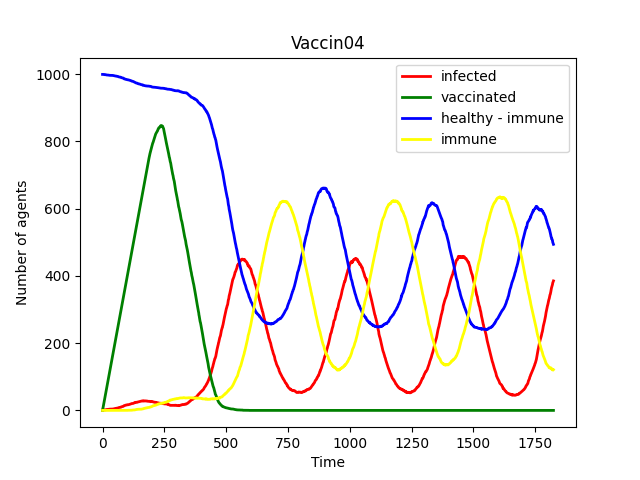
\includegraphics[width=6cm]{../Courbes/1000_agents_1_contaminé_5_ans/Vaccin04.png} }}
	\qquad
	\caption{Représentations graphique de l'évolution de l'état\\ de la population en fonction du nombre de nouveaux vaccinés par jours}

\end{figure}

C'est graphiques représentent l'évolution de l'état de la population en fonction du temps (en jours) pour un nombre de personnes qui se font vacciner chaque jour.
On observe que le fait d'avoir une partie de la population vaccinée est une bonne pratique pour réduire la transmission de la maladie. En effet, le pic de vaccination permet de
fortement retardé le pic de contamination initial.
\newpage
De plus, on peut voir que nombre de personnes qui se vaccinent chaque jour est un facteur important pour retarder le début de l'épidémie.

Par la suite, nous avons implémenté les rappels de vaccins. Nous revaccinons les agents dès lors que leur vaccin ne fait plus effet. On regarde donc le seuil minimal de personnes à vacciner par jour
pour que la maladie soit éradiquée.

\begin{figure}[h]
	\centering
	\subfloat[\centering 1 vaccination par jour]{{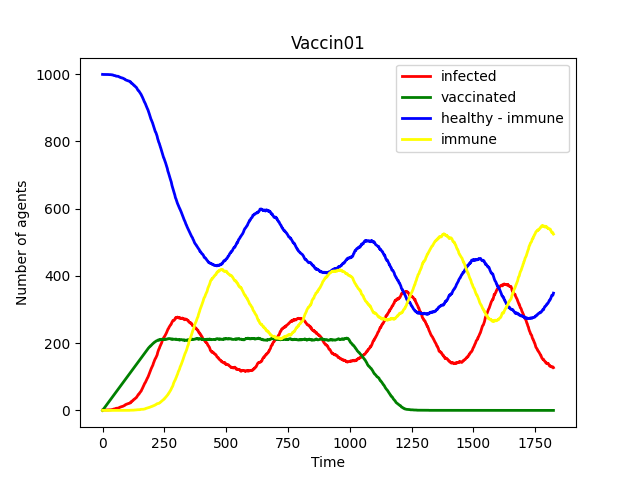
\includegraphics[width=6cm]{../Courbes/1000_agents_1_contaminé_5_ans/Vaccin01.png} }}
	\qquad
	\subfloat[\centering 3 vaccination par jour]{{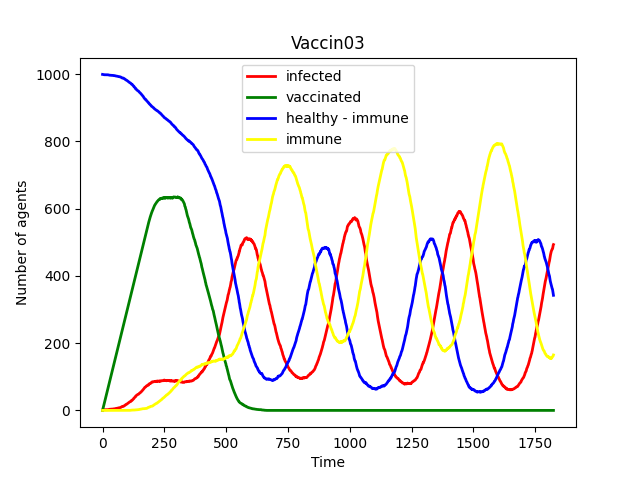
\includegraphics[width=6cm]{../Courbes/1000_agents_1_contaminé_5_ans/Vaccin03.png} }}
	\centering
	\subfloat[\centering 4 vaccination par jour]{{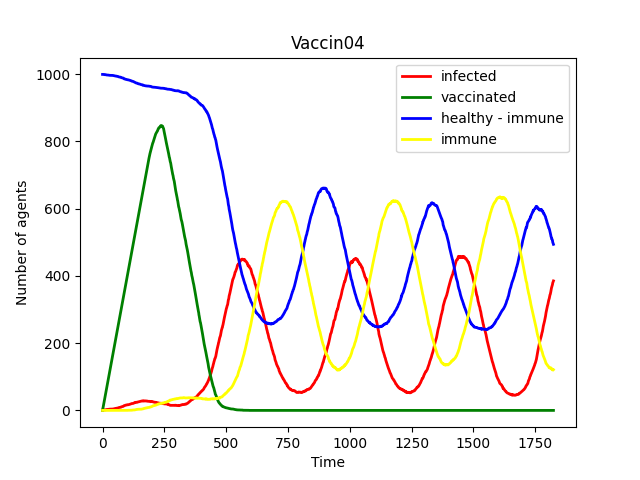
\includegraphics[width=6cm]{../Courbes/1000_agents_1_contaminé_5_ans/Vaccin04.png} }}
	\qquad
	\caption{Représentations graphique de l'évolution de l'état\\ de la population en fonction du nombre de nouveaux vaccinés par jours}

\end{figure}

Ces graphiques montrant l'évolution de l'état de la population en fonction du temps (en jours) pour un nombre de personnes qui se font vacciner chaque jour démontrent bien que
se faire vacciner régulièrement permet de très facilement éradiquer la maladie. En effet, on observe que dès trois personnes vaccinées suplémentaires par jour, la maladie ne dépasse pas les 15\% d'infectés.
Et qu'il suffit de vacciner quatres personnes par jour pour éradiquer la maladie au bout de deux ans pour une population de 1000 agents.

\newpage

Nous avons réitéré l'expérience "vaccin" mais avec un nombre d'agents contaminés à 100 à t0 pour simuler une épidémie en cours.

\begin{figure}[h]
	\centering
	\subfloat[\centering 1 vaccination par jour]{{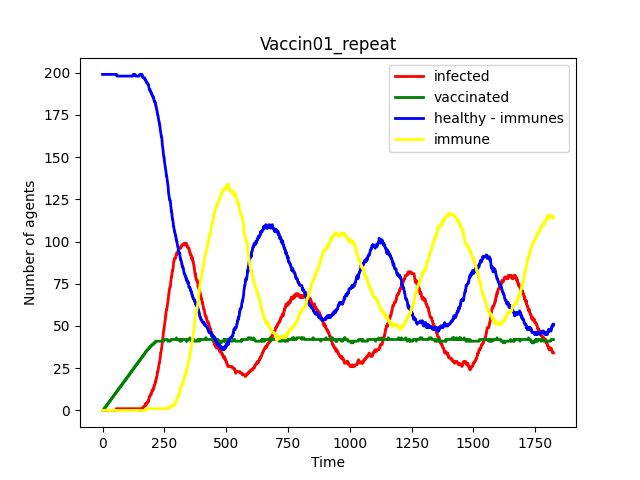
\includegraphics[width=6cm]{../Courbes/1000_agents_100_contaminé_5_ans/Vaccin01_repeat.png} }}
	\qquad
	\subfloat[\centering 3 vaccination par jour]{{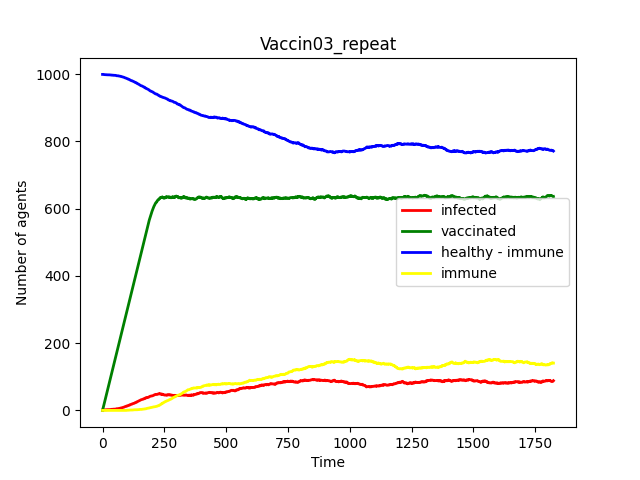
\includegraphics[width=6cm]{../Courbes/1000_agents_100_contaminé_5_ans/Vaccin03_repeat.png} }}
	\centering
	\subfloat[\centering 4 vaccination par jour]{{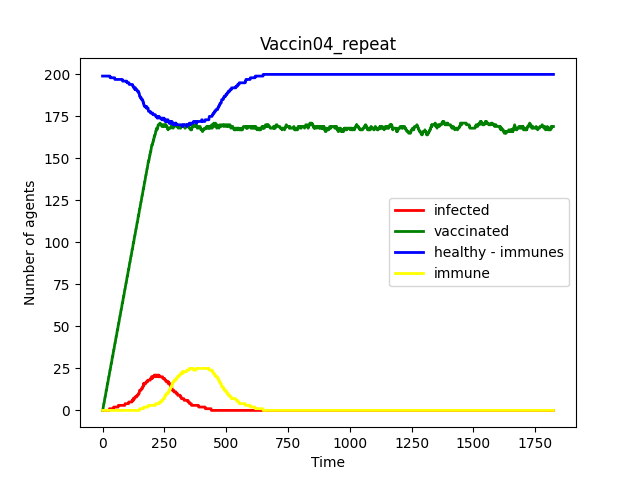
\includegraphics[width=6cm]{../Courbes/1000_agents_100_contaminé_5_ans/Vaccin04_repeat.png} }}
	\qquad
	\caption{Représentations graphique de l'évolution de l'état\\ de la population en fonction du nombre de nouveaux vaccinés par jours}

\end{figure}

On arrive aux mêmes conclusions qu'à l'expérience précédente, le vaccin est la meilleure pratique pour éradiquer la maladie et il faut vacciner au moins trois personnes par jour pour
que les résultats soient réellement significatifs.

\newpage

\subsection{Combinaisons de méthodes}

Enfin, après avoir présenté les différentes facon d'entraver la propagation d'une maladie au sein d'une population, nous avons décidé de tester différentes combinaisons de méthodes.
Nous présentons donc deux d'entre elles :

\begin{itemize}
	\item Light confinement and medium barrier gestures
	\item Mediums barrier gestures and vaccin 3 people per day with vaccin booster
\end{itemize}

\begin{figure}[h]
	\subfloat[\centering Light confinement and medium barrier gestures]{{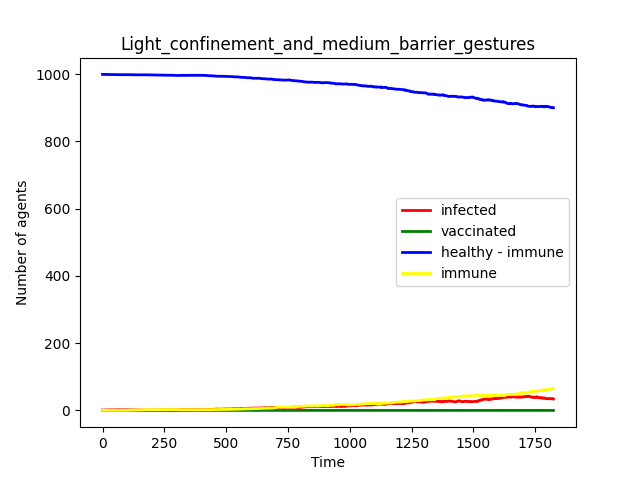
\includegraphics[width=6cm]{../Courbes/1000_agents_1_contaminé_5_ans/Light_confinement_and_medium_barrier_gestures.png} }}
	\subfloat[\centering Mediums barrier gestures and vaccin 3 people per day with vaccin booster]{{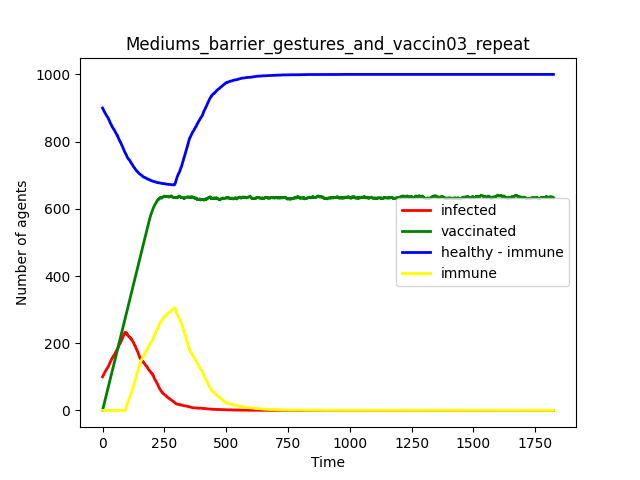
\includegraphics[width=6cm]{../Courbes/1000_agents_1_contaminé_5_ans/Mediums_barrier_gestures_and_vaccin03_repeat.png} }}
	\caption{Représentations graphique de l'évolution de l'état\\ de la population en fonction de la combinaison de méthodes}
\end{figure}

Étant donné que les méthodes combinées ici ont fait leurs preuvent individuellement, nous avons donc pu voir que les résultats sont significatifs. Cependant, pour le light confinement and le medium barrier gestures, on vois
que la maladie est plus difficile à éradiquer. Ces deux méthodes étant plus utilisée pour ralentir la propagation que pour l'éradiquer, on observe que la maladie progresse tout de même.
Tandis que Mediums barrier gestures and vaccin 3 people per day with vaccin booster ne permet même pas à la maladie d'évoluer.

\newpage

\section{Conclusion}

Après cette baterie de tests, nous sommes en mesure de définir la facon la plus efficace de contrer cette nouvelle maladie. Tout d'habord, si cette dernière est remarquée suffisement tôt,
un confinement light avec une population qui fait attention aux gestes de barrière de base, permettrait de fortement ralentir sa propagation en attendant le développemnt d'un vaccin qui permettrait de l'éradiquer .
\end{document}

